\chapter{Elastic Parameter Calculation for BCC crystal}\label{appen_bccel}
Applying a small strain ($\delta$) to the equilibrium lattice changes the total energy, and from this information, the elastic parameters are deduced. The distortion of a lattice vector follows the rule $\mathbf{R'} = \mathbf{RD}$. Here, $\mathbf{R}$ is the Bravais lattice vector, $\mathbf{R'}$ is a matrix containing the components of the distorted lattice vectors, and $\mathbf{D}$ is the symmetric distortion matrix.


By symmetry, there are only three independent elastic parameters for a cubic system (\ie, $C_{11}, C_{12}$, and $ C_{44}$).
Elastic parameters are evaluated from the total energy of the crystal, to which volume-conserving orthorhombic $[C'=(C_{11} - C_{12})/2]$ and monoclinic $(C_{44})$ distortions are applied. The relevant distortion matrices are 
%\[\begin{bmatrix}
\begin{equation}
\mathbf{D}_\text{ortho} = \label{eq:ortho}
		\begin{bmatrix}
		1+\delta_o & 0 & 0 \\
		0 & 1-\delta_o & 0 \\
		0 & 0 & \frac{1}{1-\delta_o^2}\\
		\end{bmatrix}
\end{equation}
%\end{bmatrix} \]
and
\begin{equation}
\label{eq:mono}
\mathbf{D}_\text{mono} = \begin{bmatrix}
	1 & \delta_m & 0 \\
	\delta_m & 1 & 0 \\
	0 & 0 & \frac{1}{1-\delta_m^2} \\
\end{bmatrix}.
\end{equation}
The associated total energy change for an orthorhombic distortion is 
\begin{equation}
\label{eq_ortho}
\Delta E = V(C_{11} - C_{12})\delta_o^2 + O(\delta_o^4) .
\end{equation}
For a monoclinic distortion, the energy change is
\begin{equation}
\label{eq_mono}
\Delta E = 2VC_{44}\delta_m^2 + O(\delta_m^4).
\end{equation}

\begin{figure}
	\centering
	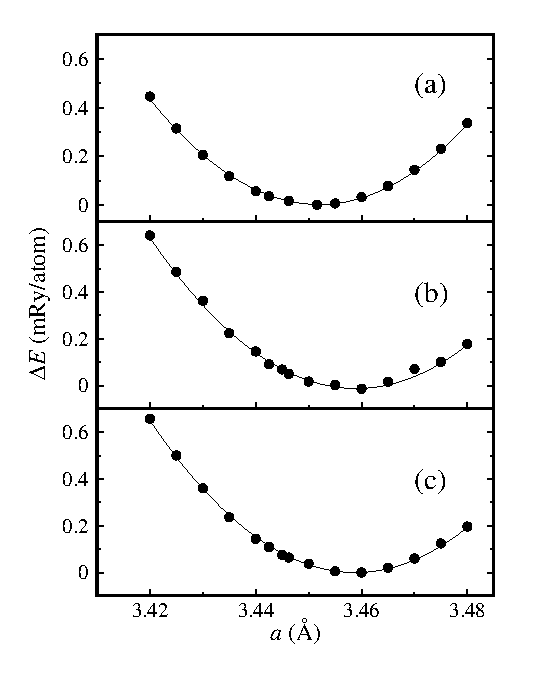
\includegraphics[width=4.25 in]{figure_bulk}
    \caption[Energy as a function of lattice parameters for \textgamma-uranium.]{Energy as a function of lattice parameters for \textgamma-uranium. (a)~Our work~\cite{iasir2020pseudopotential} with a $k$-point mesh of $30\times30\times30$; (b)~Pseudopotential from PS library~\cite{dal2014pseudopotentials, pp1}
 with a $k$-point mesh of $30\times30\times30$; (c)~Pseudopotential from PS library~\cite{dal2014pseudopotentials, pp1}
 with $42\times42\times42$ $k$-point mesh.}
	\label{fig:bulkgamma}
\end{figure}

\begin{figure}
	\centering
	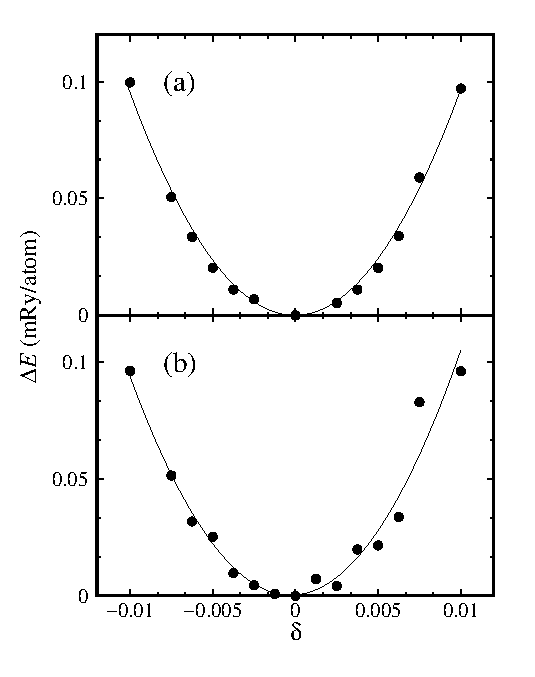
\includegraphics[width=3.25 in]{figure_mono}
    \caption[Changes in the strain energy as a function of strain $(\delta)$ for monoclinic distortions of \textgamma-uranium ]{Changes in the strain energy as a function of strain $(\delta)$ for monoclinic distortions of \textgamma-uranium (Eq.~\eqref{eq:mono} and Eq.~\eqref{eq_mono}). (a)~Our work~\cite{iasir2020pseudopotential}; (b)~Pseudopotential from the PS library~\cite{dal2014pseudopotentials, pp1}. Increasing the $k$-points does not improve the smoothness of plot (b).}
\label{fig:monogamma}
\end{figure}


\begin{figure}
	\centering
	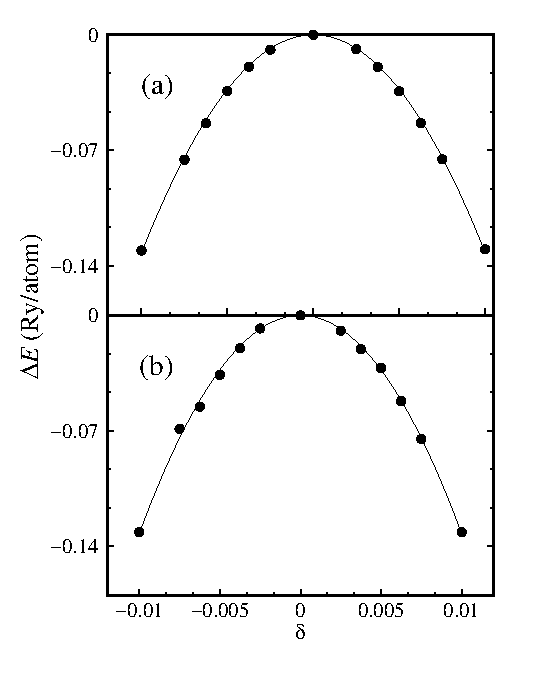
\includegraphics[width=3.25 in]{figure_ortho}
    \caption[Changes in the strain energy as a function of strain $(\delta)$ for orthorhombic distortions of \textgamma-uranium ]{Changes in the strain energy as a function of strain $(\delta)$ for orthorhombic distortions of \textgamma-uranium (Eq.~\eqref{eq:ortho} and Eq.~\eqref{eq_ortho}). (a)~Our work~\cite{iasir2020pseudopotential}; (b)~Pseudopotential from the PS library~\cite{dal2014pseudopotentials, pp1}.}
	\label{fig:orthogamma}
\end{figure}

A sample python code to generate and run the distorted lattice in quantum espresso is shown below.

%\newpage
\bibliographystyle{unsrt}
\bibliography{abbreviated,comp,umox}

\newpage
\lstset{style=pythn}
\begin{lstlisting}
import os, subprocess
from glob import glob
import re
import matplotlib.pyplot as plt 
import numpy as np

def matprintf(x):
    for i in range(len(x)):
         print ('{:16.13f} {:16.13f} {:16.13f}'.format(x[i][0],x[i][1],x[i][2]))

#d = np.array([3.42, 3.43, 3.44, 3.455, 3.45, 3.465, 3.46, 3.475, 3.47, 3.48, 3.445, 3.4425])
d = np.array([0,0.01,-0.01,0.005,-0.005,0.0075,-0.0075,0.00625,-0.00625,0.0025,-0.0025,0.00375,-0.00375,0.00125,-0.00125,0.02,-0.02])
    
        # Run with different ecutwfc
for i in range(len(d)):
    dd = d[i]
    A12 = dd
    A21 = dd
    A33 = np.float128(1/((1-dd**2)))
     #crystal axis for bcc
    R = np.array([[-0.5,0.5,0.5],[0.5,-0.5,0.5],[0.5,0.5,-0.5]],dtype=np.float128)
    #distortion matrix for monoclinic distortion
    Dmono = np.array([[1,A12,0.0],[A21,1,0.0],[0.0,0.0,A33]],dtype=np.float128)
    Rprime = np.matmul(R,Dmono)


    filename = 'U_qepp_gamma.scf' 
    pseudo = '/home/scruffy/rafi/Desktop/rafi/quantum_espresso/supercell_study/pp_dir'
    with open(filename + str(d[i]) + '.in','w') as f:
        f.write("&control\n")
        f.write("title = 'U_gamma'\n")
        f.write("    calculation = 'relax'\n")
        f.write("    restart_mode = 'from_scratch'\n")
        f.write("    pseudo_dir = '{:s}' \n".format(pseudo))
        f.write("    outdir = '{:s}'\n".format(pseudo))
        f.write("    prefix = 'gammaU'\n")
        f.write("    etot_conv_thr = 1.0e-8\n")
        f.write("    forc_conv_thr = 1.0e-8 \n")
        #f.write("    tstress = .true.\n")
                #f.write("    tprnfor = .true.\n")
        f.write("/\n")
        f.write(" ")
        f.write("&system\n")
        f.write("    ibrav = 0\n")
        f.write("       A = 3.459\n")
        #f.write("        A = {:3.10f}\n" .format(d[i]))
        f.write("    nat = 1\n")
        f.write("    ntyp = 1\n")
        f.write("    ecutwfc = 50 \n")
        f.write("    ecutrho = 250 \n")
        f.write("    smearing = 'methfessel-paxton'\n")
                #f.write("    smearing = 'gauss'\n")
                #f.write("    degauss = 0.01\n")
        f.write("/\n")
        f.write(" ")
        f.write("&electrons\n")
        f.write("    diagonalization = 'david'\n")
                #f.write("    conv_thr = 1.0e-8\n")
                #f.write("    mixing_beta = 0.7\n")
        f.write("/\n")
        f.write(" ")
        f.write("&IONS\n")
        f.write("/\n")
        f.write(" ")
        f.write("&CELL\n")
        f.write("/\n")
        f.write("CELL_PARAMETERS {alat} \n")
        #f.write("  -0.5    0.5   0.5 \n")
        #f.write("   0.5   -0.5   0.5 \n")
        #f.write("   0.5    0.5  -0.5 \n")
    
        for j in range (len(Rprime)) :
                 f.write ('{:16.13f} {:16.13f} {:16.13f} \n'.format(Rprime[j][0],Rprime[j][1],Rprime[j][2]))
    
        f.write(" \n")
        f.write("ATOMIC_SPECIES\n")
        f.write("U 238.029  U.GGA-PBE-paw.UPF\n")
        f.write(" \n")
        f.write("ATOMIC_POSITIONS {crystal}\n")
        f.write("U  0.000  0.000 0.000\n")
        f.write(" \n")
        f.write("K_POINTS automatic\n")
        f.write("35 35 35 0 0 0\n")
    command = ('mpiexec -n 8 pw.x -i ' + filename + str(d[i]) + '.in > ' + filename + str(d[i]) + '.out' )
    print(command)
    p = subprocess.Popen(command, shell=True)
    p.wait()

\end{lstlisting}


